\documentclass[graybox, envcountchap]{svmult}

% --- kodiranje, jezik, pisave -----------------------------------------
\usepackage[utf8]{inputenc}
\usepackage[T1]{fontenc}
\usepackage[slovene]{babel}
\usepackage{mathptmx}          % Times Roman
\usepackage{helvet}            % Helvetica
\usepackage{courier}           % Courier

% --- matematika -------------------------------------------------------
\usepackage{amsmath}
\usepackage{amssymb}
\usepackage{physics}           % \ket, \bra, \braket, \expval ...

% --- slike, tabele, diagrami ------------------------------------------
\usepackage{graphicx}
\usepackage{caption}
\usepackage{subcaption}
\usepackage{float}
\usepackage{booktabs}          % \toprule, \midrule, \bottomrule
\usepackage{multirow}
\usepackage{tabularx}
\usepackage[separate-uncertainty=true]{siunitx}
\sisetup{output-decimal-marker={,}}
\usepackage{tikz}
\usepackage{quantikz}          % kvantna vezja

% --- programska koda --------------------------------------------------
\usepackage{xcolor}
\usepackage{listings}
\lstset{
  basicstyle=\ttfamily\footnotesize,
  keywordstyle=\color{blue!60!black}\bfseries,
  commentstyle=\color{gray},
  stringstyle=\color{red!50!black},
  numbers=left, numberstyle=\tiny\color{gray},
  frame=single, breaklines=true, columns=fullflexible,
  showstringspaces=false, captionpos=b
}

% --- ostalo -----------------------------------------------------------
\usepackage{multicol}
\usepackage[bottom]{footmisc}
\usepackage{comment}
\usepackage{csquotes}          % \enquote{...}
\usepackage[numbers,square,sort&compress]{natbib} % številčni sklici [1--3]
\usepackage{xurl}
\usepackage[hidelinks]{hyperref}

\setlocalecaption{slovene}{theorem}{Izrek}
\setlocalecaption{slovene}{definition}{Definicija}

\begin{document}

%%%%%%%%%%%%%%%%%%%%%%%%%%%%%%%%%%%%%%%%%%%%%%%%%%%%%%%%%%%%%%%%%%%%%%
% Začetek dejanskega poglavja - besedilo pred tem izbrisi pred oddajo
%%%%%%%%%%%%%%%%%%%%%%%%%%%%%%%%%%%%%%%%%%%%%%%%%%%%%%%%%%%%%%%%%%%%%%

\graphicspath{{img/}}   % v zborniku: \graphicspath{{Skupina10/img/}}

\title{Vpliv ravni optimizacije prevajalnika Qiskit na reverzibilna vezja na šumnem kvantnem procesorju IBM}
\titlerunning{Ravni optimizacije Qiskit in reverzibilna vezja}
\author{Matej Mlakar}
\maketitle

\abstract{%
% TODO: povzetek (napišem čisto na koncu)
}


\section{Uvod}
\label{g10:sec:uvod}

% TODO: uvod (napišem po rezultatih in razpravi)

% TODO: v uvod dodaj opis Toffolijevih in Fredkinovih vrat
% ter poln funkcijski nabor (premaknjeno iz Metod). Prejšnje besedilo:
% Toffolijeva vrata negirajo ciljni bit,
% če sta oba kontrolna bita 1.
% Fredkinova vrata zamenjata dva bita,
% če je kontrolni bit 1.
% Obe funkciji tvorita poln funkcijski nabor~\cite{reversible:mraz}.

% TODO: splošni odstavek o prevajalniku premakni iz Metod
% (razdelek g10:sec:poskusi, od "Prevajalnik (angl. transpiler)"
% do "a prevajanje traja dlje") v uvod.
% - V uvod: šest faz, postavitev in usmerjanje (angl. izraza
%   ob prvi omembi), SABRE in izbira SWAP, prevod v osnovna vrata
%   in optimizacija, višje ravni = boljša vezja, daljše prevajanje.
% - V Metodah ostane stavek "Algoritem je naključen, zato ga
%   prevajalnik požene večkrat in obdrži poskus z najmanj vrati
%   SWAP (preverili smo v izvorni kodi Qiskita)." Prestavi ga
%   k odstavku z 10 semeni (utemeljuje semena).
% - Pred seznamom ravni dodaj: "Faze prevajalnika smo opisali
%   v razdelku~\ref{g10:sec:uvod}. Ravni optimizacije se
%   v Qiskit 2.6.2 razlikujejo takole:"

\begin{svgraybox}
\textbf{Raziskovalno vprašanje.} Kako vpliva raven optimizacije prevajalnika Qiskit (0--3) na število dvokubitnih vrat reverzibilnih vezij in kako to vpliva na verjetnost pravilnega rezultata na šumnem procesorju IBM?

\textbf{Pričakovani rezultat.} Prehod z ravni 0 na raven 1 zmanjša število dvokubitnih vrat za več kot 30~\% in opazno izboljša pravilnost. Razlika med ravnema 2 in 3 je majhna: manj kot 10~\% v številu dvokubitnih vrat in manj kot 3 odstotne točke v pravilnosti.
\end{svgraybox}


\section{Metode}
\label{g10:sec:metode}

\subsection{Orodja in nastavitve}
\label{g10:sec:orodja}

Vezja smo zgradili in prevedli s knjižnico Qiskit~\cite{qiskit2024}.
Simulirali smo jih s Qiskit Aer,
na procesor pa poslali s Qiskit IBM Runtime.
Različice paketov so v datoteki \texttt{requirements.txt}.
Koda, rezultati in navodila za ponovitev so v repozitoriju
\url{https://github.com/JavaTerminator20/npmp-seminar-1}.

Vezja smo prevajali na vseh štirih ravneh optimizacije (0--3).
Pognali smo jih na simulatorjih
in na kvantnem procesorju \texttt{ibm\_marrakesh}.
Šumni model simulatorja smo zgradili iz kalibracije tega procesorja
19.~11.~2026 ob 12.13.

Procesor smo uporabljali z brezplačnim računom IBM Quantum
(angl.\ Open Plan).
Spada v družino Heron r2 in ima 156 kubitov
v mreži \enquote{heavy-hex}~\cite{g10:ibm_processor_types}.
Vsak kubit je povezan z največ tremi sosedi.
Osnovna vrata so CZ, RZ, SX in X,
edina dvokubitna vrata so torej CZ.
Ker IBM procesor med dnevom znova kalibrira,
smo shranili vse uporabljene kalibracije.

Strukturne metrike smo izračunali za \texttt{FakeMarrakesh},
posnetek istega procesorja.
Priložen je paketu Qiskit IBM Runtime, zato
prevajanje zanj ne potrebuje računa IBM in je ponovljivo.
Povezljivost je enaka kot pri pravem procesorju.
V seriji B smo uporabili iste postavitve
kot na pravem procesorju.
V obeh serijah je število dvokubitnih vrat
povsod enako kot pri prevajanju za pravi procesor.


\subsection{Zasnova poskusov}
\label{g10:sec:poskusi}

Uporabili smo štiri reverzibilna vezja (tabela~\ref{g10:tab:vezja}).
Polni seštevalnik je sestavljen iz Toffolijevih vrat in vrat CNOT
(slika~\ref{g10:fig:polni}).
Dvobitni Cuccarov seštevalnik~\cite{g10:cuccaro2004}
smo zgradili ročno iz blokov MAJ in UMA,
saj je razred \texttt{CDKMRippleCarryAdder} v Qiskit 2.6.2 zastarel.
Tako tudi natančno vemo, katera vrata vstopijo v prevajalnik.

\begin{table}[htbp]
\caption{Reverzibilna vezja v poskusih.
Vsako vezje smo pognali za vse vhode.}
\label{g10:tab:vezja}
\centering
\small
\begin{tabular}{lrrl}
\toprule
Vezje & Kubiti & Vhodi & Gradnja \\
\midrule
Toffoli & 3 & 8 & \texttt{ccx} \\
Fredkin & 3 & 8 & \texttt{cswap} \\
polni seštevalnik & 4 & 8 & 2 Toffoli + 2 CNOT \\
Cuccaro (dvobitni) & 6 & 16 & 2 MAJ + CNOT + 2 UMA \\
\midrule
skupaj & & 40 & \\
\bottomrule
\end{tabular}
\end{table}

Vsi kubiti začnejo v stanju $\ket{0}$.
Vhod nastavimo z vrati X,
nato sledita ukaz \texttt{barrier} in jedro vezja.
Ukaz \texttt{barrier} prevajalniku prepreči,
da bi vrata X združil z jedrom.
Sicer bi lahko vezje poenostavil za konkreten vhod.
Jedro je tako po prevajanju za vse vhode enako.
Reverzibilno vezje vsak vhod preslika v natanko en izhod.
Pričakovani izhod zato izračunamo klasično, iz pravilnostne tabele.
Na idealnem simulatorju je vseh 40 vhodov dalo pravilen izhod.
S tem smo preverili tudi vrstni red bitov v Qiskitu.

\begin{figure}[htbp]
\centering
\begin{quantikz}[row sep={0.75cm,between origins}, column sep=0.3cm]
\lstick{$q_0\colon \ket{0}$} & \gate{X^{a}} \slice{} & \ctrl{1} & \ctrl{1} & \qw & \qw & \meter{} & \setwiretype{n} \rstick{$a$} \\
\lstick{$q_1\colon \ket{0}$} & \gate{X^{b}} & \ctrl{2} & \targ{} & \ctrl{1} & \ctrl{1} & \meter{} & \setwiretype{n} \rstick{$a \oplus b$} \\
\lstick{$q_2\colon \ket{0}$} & \gate{X^{c_\text{in}}} & \qw & \qw & \ctrl{1} & \targ{} & \meter{} & \setwiretype{n} \rstick{$s$} \\
\lstick{$q_3\colon \ket{0}$} & \qw & \targ{} & \qw & \targ{} & \qw & \meter{} & \setwiretype{n} \rstick{$c_\text{out}$}
\end{quantikz}
\caption{Polni seštevalnik s pripravo vhoda
in ukazom \texttt{barrier} (črtkano).
Vrata $X^{a}$ se izvedejo le, če je $a = 1$.
Na izhodu je $s$ vsota, $c_\text{out}$ pa prenos.}
\label{g10:fig:polni}
\end{figure}

Prevajalnik (angl.\ transpiler) vezje prilagodi procesorju
v šestih fazah~\cite{g10:qiskit_transpiler_stages}.
Postavitev (angl.\ layout) določi,
na katerem fizičnem kubitu bo logični kubit.
Usmerjanje (angl.\ routing) doda vrata SWAP,
kadar dvokubitna vrata delujejo na nepovezanih kubitih.
Za postavitev in usmerjanje Qiskit uporablja
algoritem SABRE~\cite{g10:li2019sabre}.
Ta vrata SWAP izbira tako, da zmanjša razdaljo
med kubiti naslednjih dvokubitnih vrat.
Algoritem je naključen~\cite{g10:qiskit_transpiler_stages},
zato ga prevajalnik požene večkrat
in obdrži poskus z najmanj vrati SWAP
(preverili smo v izvorni kodi Qiskita).
Nato prevajalnik vezje prevede v osnovna vrata in optimizira.
Višje ravni optimizacije dajo boljša vezja,
a prevajanje traja dlje~\cite{g10:qiskit_optimization}.
Ravni se razlikujejo takole:

\begin{itemize}
\item \textbf{Raven 0:}
Logični kubit $i$ postavi na fizični kubit $i$,
usmerja s \texttt{SabreSwap}.
Faze optimizacije ni.
\item \textbf{Raven 1:}
Če trivialna postavitev potrebuje vrata SWAP,
poišče postavitev brez njih (\texttt{VF2Layout}).
Sicer uporabi algoritem SABRE~\cite{g10:li2019sabre} s 5 poskusi.
Po usmerjanju izbere kubite z manjšimi napakami
(\texttt{VF2PostLayout}).
Nato združuje enokubitna vrata in odstranjuje pare inverznih vrat,
dokler se vezje spreminja.
\item \textbf{Raven 2:}
Trivialne postavitve ne poskusi, SABRE ima 20 poskusov.
Vezje krajša že pred postavitvijo,
pri tem upošteva tudi komutativnost vrat.
Bloke dvokubitnih vrat enkrat na novo sintetizira.
Obdrži boljšo različico, predvsem po številu dvokubitnih vrat
(\texttt{TwoQubit\allowbreak Peephole\allowbreak Optimization}).
\item \textbf{Raven 3:}
SABRE izvede dvakrat več iteracij.
Ponovna sinteza blokov je v zanki,
ki vrne najboljše najdeno vezje (\texttt{MinimumPoint}).
Na koncu še enkrat izbere kubite z manjšimi napakami.
\end{itemize}

Izboljšanje z ravni 0 na 1 je
vsota boljše postavitve in optimizacije vrat.
Da ju ločimo, smo izvedli dve seriji.
V seriji A postavitev izbere prevajalnik,
v seriji B pa vse ravni dobijo isto začetno postavitev
(\texttt{initial\_layout}).
Prevajalnik takrat preskoči vse prehode za postavitev,
tudi \texttt{VF2PostLayout}.
Postavitev B smo za vsako vezje izbrali enkrat,
s požrešnim postopkom, ki išče povezane kubite z najmanjšo vsoto
napak vrat CZ in napak meritve.
Tako fiksna postavitev nobene ravni ne kaznuje.
Napake so iz kalibracije 19.~11.~2026 ob 8.37.

Vsako kombinacijo vezja, serije in ravni
smo prevedli z 10 semeni prevajalnika
in rezultate povprečili.
Raztros podamo s standardnim odklonom.

Vezja, prevedena za \texttt{ibm\_marrakesh},
smo pognali na treh platformah:
\begin{itemize}
\item \emph{Idealni simulator} (\texttt{AerSimulator} brez šuma) je kontrola.
Pognali smo seme 0 s 1000 ponovitvami (angl.\ shots).
Pričakujemo $P_\text{pravilno} = 1$.
\item \emph{Šumni model} (\texttt{AerSimulator.from\_backend})
vsebuje napake vrat, razpad kubitov in napake meritve
iz kalibracije procesorja.
Drugih pojavov, npr.\ presluha med kubiti, ne vsebuje.
Pognali smo vse kombinacije,
3200 vezij z 2000 ponovitvami.
\item \emph{Kvantni procesor}: vsaka serija je ena naloga
s 160 vezji ($40$ vhodov $\times\,4$ ravni) in 1000 ponovitvami.
Ker je čas omejen, smo pognali le eno seme,
tisto z mediano števila dvokubitnih vrat.
Tako poženemo tipičen primer, ne najboljšega ali najslabšega.
\end{itemize}
Na procesorju smo izklopili dinamično razklapljanje
(angl.\ dynamical decoupling)
in naključno sukanje vrat (angl.\ twirling), zato
da merimo le vpliv prevajalnika.


\subsection{Metrike}
\label{g10:sec:metrike}

Na prevedenem vezju merimo število uporabljenih kubitov,
število dvokubitnih vrat (CZ), globino,
skupno število vrat in čas prevajanja (klic \texttt{pm.run}).
Meritev in ukazov \texttt{barrier} ne štejemo.
Glavna metrika je število dvokubitnih vrat.
Ta imajo večjo napako in daljše trajanje kot enokubitna vrata.
Število dvokubitnih vrat je za vse vhode istega vezja enako,
kar smo preverili na vseh pognanih vezjih.
Globina se zaradi vrat X razlikuje za največ 1.
Zato metrike računamo na vezju z vhodom $0\ldots0$.

Verjetnost pravilnega rezultata za eno vezje je
\begin{equation}
P_\text{pravilno} = \frac{1}{|V|} \sum_{v \in V} \frac{N_\text{pravilno}(v)}{N} ,
\label{g10:eq:ppravilno}
\end{equation}
kjer je $V$ množica vhodov vezja, $N$ število ponovitev
in $N_\text{pravilno}(v)$ število ponovitev s pravilnim izhodom.
Izhod je pravilen le, če se ujemajo vsi izmerjeni biti.
Pri šumnem modelu rezultat povprečimo še čez semena.
Standardna napaka na en vhod je $\sqrt{P(1-P)/N}$,
kar je največ 1,1 odstotne točke pri $N = 2000$
in 1,6 odstotne točke pri $N = 1000$.

Spremembo med ravnema optimizacije $i$ in $j$ izračunamo kot
\begin{equation}
\Delta n_{i \to j} = \frac{\bar{n}_i - \bar{n}_j}{\bar{n}_i} \cdot 100~\% ,
\qquad
\Delta P_{i \to j} = \left( P_j - P_i \right) \cdot 100 ,
\label{g10:eq:spremembe}
\end{equation}
kjer je $\bar{n}_i$ povprečno število dvokubitnih vrat na ravni $i$
in $P_i$ verjetnost $P_\text{pravilno}$ na ravni $i$.
$\Delta P$ je v odstotnih točkah,
pozitivna vrednost pri obeh pomeni izboljšanje.
Prvo hipotezo preverimo z $\Delta n_{0\to1}$ in $\Delta P_{0\to1}$,
drugo z absolutnima vrednostma $\Delta n_{2\to3}$ in $\Delta P_{2\to3}$.
[TODO: prijava ne določa praga za \enquote{opazno} izboljšanje
pravilnosti v prvi hipotezi; določi merilo.]
Za povprečje čez vezja najprej povprečimo števila vrat
in $P_\text{pravilno}$, nato izračunamo spremembo.


\section{Rezultati}
\label{g10:sec:rezultati}

\subsection{Število dvokubitnih vrat}
\label{g10:sec:rez_vrata}

Povprečno število dvokubitnih vrat je v tabeli~\ref{g10:tab:vrata}.
Pred prevajanjem ima Toffolijevo vezje 6 vrat CNOT,
enako kot standardna razgradnja~\cite{nielsen2010}.
Tudi v ostalih vezjih vsaka Toffolijeva vrata
prispevajo po 6 vrat CNOT.

\begin{table}[htbp]
\caption{Povprečno število dvokubitnih vrat čez 10 semen prevajalnika.
Stolpec \enquote{pred} je vezje, razgrajeno v vrata CNOT
in enokubitna vrata pri polni povezljivosti, brez optimizacije.
Številke 0--3 so ravni optimizacije.}
\label{g10:tab:vrata}
\centering
\small
\setlength{\tabcolsep}{4pt}
\begin{tabular}{lrrrrrrrrr}
\toprule
 & & \multicolumn{4}{c}{serija A} & \multicolumn{4}{c}{serija B} \\
\cmidrule(lr){3-6} \cmidrule(lr){7-10}
Vezje & pred & 0 & 1 & 2 & 3 & 0 & 1 & 2 & 3 \\
\midrule
Toffoli & $6{,}0$ & $12{,}0$ & $9{,}0$ & $7{,}4$ & $7{,}4$ & $12{,}0$ & $12{,}0$ & $9{,}0$ & $9{,}0$ \\
Fredkin & $8{,}0$ & $14{,}9$ & $11{,}0$ & $10{,}0$ & $10{,}0$ & $14{,}9$ & $14{,}0$ & $11{,}0$ & $11{,}0$ \\
polni seštevalnik & $14{,}0$ & $27{,}8$ & $16{,}0$ & $14{,}8$ & $14{,}8$ & $26{,}6$ & $22{,}0$ & $17{,}2$ & $17{,}2$ \\
Cuccaro & $33{,}0$ & $67{,}8$ & $53{,}7$ & $45{,}4$ & $45{,}6$ & $68{,}4$ & $60{,}0$ & $48{,}0$ & $48{,}0$ \\
\midrule
povprečje & $15{,}3$ & $30{,}6$ & $22{,}4$ & $19{,}4$ & $19{,}5$ & $30{,}5$ & $27{,}0$ & $21{,}3$ & $21{,}3$ \\
\bottomrule
\end{tabular}
\end{table}

Raven 0 število vrat približno podvoji,
ker usmerjanje doda vrata SWAP.
Raven 1 ga zmanjša za 20,8 do 42,4~\%,
v povprečju za 26,8~\% (tabela~\ref{g10:tab:spremembe}).
V seriji A raven 2 odstrani
še 1,0 do 8,3 vrat.
Raven 3 števila vrat ne zmanjša več.
V 79 od 80 kombinacij vezja, serije in semena
dasta ravni 2 in 3 enako število vrat.
Tudi na ravni 3 ostane več vrat kot pred prevajanjem.
Pri Toffoliju najboljše seme da 7 vrat, povprečje je 7,4.
To je cena omejene povezljivosti procesorja.

Raztros med semeni je največji na ravni 0,
do 3,9 vrat pri Cuccarovem seštevalniku.
Na višjih ravneh je največ 1,3 vrat.
V seriji A se globina z ravni 0 na 3
zmanjša za 46 do 61~\%,
pri Cuccaru npr.\ z 266,7 na 145,0.
Povprečni čas prevajanja je bil
na vseh ravneh pod 6~ms,
zato pri tako majhnih vezjih ni pomemben.

V seriji B imajo vse ravni isto postavitev.
Prehod z ravni 0 na 1 tu zmanjša število vrat
le za 11,4~\%, pri Toffoliju sploh ne.
Večji del izboljšanja v seriji A
torej prispeva boljša postavitev, ne optimizacija vrat.
Na ravneh 1--3 ima serija B
več vrat kot serija A.
Postavitev, izbrana po napakah kubitov,
torej zahteva več vrat kot postavitev,
ki jo izbere prevajalnik.


\subsection{Verjetnost pravilnega rezultata}
\label{g10:sec:rez_pravilnost}

Tabela~\ref{g10:tab:pravilnost} podaja $P_\text{pravilno}$
na šumnem modelu in na kvantnem procesorju.
Nalogi na procesorju sta tekli 19.~11.~2026.

\begin{table}[htbp]
\caption{Verjetnost pravilnega rezultata $P_\text{pravilno}$ v \%.
Šumni model: povprečje čez 10 semen.
Procesor: eno seme, tisto z mediano števila dvokubitnih vrat.
Številke 0--3 so ravni optimizacije.}
\label{g10:tab:pravilnost}
\centering
\small
\setlength{\tabcolsep}{4pt}
\begin{tabular}{llrrrrrrrr}
\toprule
 & & \multicolumn{4}{c}{serija A} & \multicolumn{4}{c}{serija B} \\
\cmidrule(lr){3-6} \cmidrule(lr){7-10}
Vezje & Platforma & 0 & 1 & 2 & 3 & 0 & 1 & 2 & 3 \\
\midrule
\multirow{2}{1.6cm}{Toffoli} & šumni model & $94{,}2$ & $95{,}4$ & $95{,}8$ & $96{,}0$ & $94{,}1$ & $94{,}3$ & $95{,}0$ & $95{,}0$ \\
 & procesor & $81{,}0$ & $93{,}3$ & $93{,}3$ & $94{,}6$ & $91{,}0$ & $91{,}5$ & $92{,}4$ & $91{,}6$ \\
\addlinespace
\multirow{2}{1.6cm}{Fredkin} & šumni model & $93{,}6$ & $95{,}0$ & $95{,}2$ & $95{,}3$ & $93{,}4$ & $94{,}0$ & $94{,}6$ & $94{,}6$ \\
 & procesor & $79{,}7$ & $92{,}7$ & $92{,}7$ & $94{,}4$ & $91{,}3$ & $91{,}7$ & $91{,}7$ & $91{,}9$ \\
\addlinespace
\multirow{2}{1.6cm}{polni seštevalnik} & šumni model & $89{,}8$ & $90{,}9$ & $91{,}1$ & $93{,}6$ & $89{,}2$ & $90{,}5$ & $91{,}0$ & $91{,}0$ \\
 & procesor & $73{,}4$ & $89{,}3$ & $89{,}6$ & $85{,}6$ & $75{,}6$ & $77{,}3$ & $78{,}8$ & $78{,}0$ \\
\addlinespace
\multirow{2}{1.6cm}{Cuccaro} & šumni model & $78{,}1$ & $81{,}5$ & $82{,}4$ & $83{,}9$ & $74{,}4$ & $77{,}2$ & $79{,}2$ & $79{,}2$ \\
 & procesor & $56{,}6$ & $60{,}4$ & $62{,}4$ & $61{,}7$ & $26{,}1$ & $29{,}6$ & $30{,}2$ & $30{,}6$ \\
\bottomrule
\end{tabular}
\end{table}

Na idealnem simulatorju je vseh 320 prevedenih vezij
dalo $P_\text{pravilno} = 1$.
Prevajalnik torej na nobeni ravni ni pokvaril izračuna.

Na šumnem modelu v seriji A $P_\text{pravilno}$
pri vseh vezjih narašča z ravnjo.
Spremembe pa so majhne.
Z ravni 0 na 1 se $P_\text{pravilno}$ poveča
v povprečju za 1,8 odstotne točke (o.\,t.),
z ravni 2 na 3 pa za 1,1~o.\,t.
Raztros med semeni je največ 1,1~o.\,t.
Pri polnem seštevalniku da raven 3 za 2,5~o.\,t. več
kot raven 2, čeprav imata pri vseh semenih
enako število dvokubitnih vrat.
V seriji B, kjer so kubiti pri vseh ravneh isti,
dasta ravni 2 in 3 enak $P_\text{pravilno}$.
Razlika v seriji A torej izvira iz izbire kubitov.

Na procesorju je skok z ravni 0 na 1
precej večji,
v povprečju 11,2~o.\,t.
Raven 0 je pri vseh vezjih najslabša.
Med ravnmi 1--3 so razlike manjše in nimajo enotne smeri.
Pri polnem seštevalniku je raven 3
za 4,1~o.\,t. slabša od ravni 2,
čeprav imata na pognanem semenu obe 14 vrat.
Pri 8 vhodih in 1000 ponovitvah
je standardna napaka $P_\text{pravilno}$ največ 0,6~o.\,t.

Za primerjavo s procesorjem iz šumnega modela vzamemo
le seme, ki smo ga pognali na procesorju.
Od povprečja čez vsa semena se razlikuje za največ 0,8~o.\,t.
Procesor je povsod slabši od šumnega modela.
V seriji A je pri Toffoliju in Fredkinu
razlika na ravneh 1--3
le 0,9 do 2,6~o.\,t.,
na ravni 0 pa 13,1 in 14,1~o.\,t.
Pri Cuccaru je razlika na vseh ravneh okoli 21~o.\,t.

V seriji B se $P_\text{pravilno}$
z ravni 0 na 1 poveča
le za 1,2~o.\,t. na šumnem modelu
in za 1,5~o.\,t. na procesorju.
Procesor je tu pri seštevalnikih precej slabši.
Cuccaro doseže le 26,1 do 30,6~\%,
šumni model pa 74,4 do 79,2~\%.
Razlika med modelom in procesorjem
je pri vseh ravneh skoraj enaka,
pri Cuccaru med 47,6 in 49,0~o.\,t.
Vse ravni tu tečejo na istih kubitih,
zato upad ni posledica ravni optimizacije.
Šumni model, zgrajen iz iste kalibracije kot naloga B,
tega upada ne napove.


\subsection{Povezava med številom vrat in pravilnostjo}
\label{g10:sec:rez_povezava}

Slika~\ref{g10:fig:vrata_P} prikazuje $P_\text{pravilno}$
v odvisnosti od števila dvokubitnih vrat.
Osi slike nista linearni.
Na linearnih oseh bi se točke majhnih vezij,
ki imajo malo vrat in $P_\text{pravilno}$ blizu 100~\%,
prekrivale v zgornjem levem kotu.
Točke šumnega modela ležijo na eni padajoči krivulji.
Pri Toffoliju in Fredkinu (7 do 17 vrat)
je $P_\text{pravilno}$ med 92,5 in 96,1~\%,
pri Cuccaru (43 do 75 vrat)
pa med 73,2 in 84,7~\%.
Na šumnem modelu je število dvokubitnih vrat
torej dober napovednik za $P_\text{pravilno}$.

\begin{figure}[htbp]
\centering
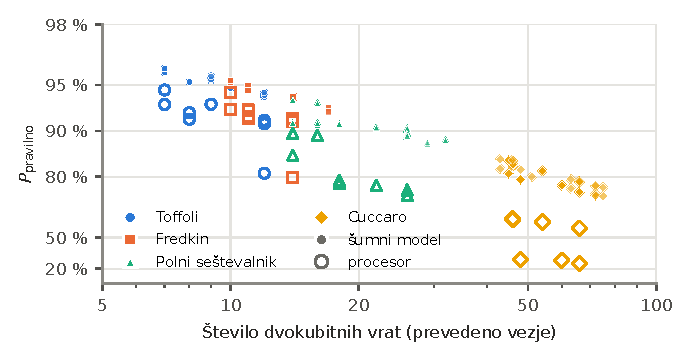
\includegraphics[width=\textwidth]{graf3_vrata_proti_P_v3.pdf}
\caption{Število dvokubitnih vrat in $P_\text{pravilno}$
za vse zagone obeh serij.
Polne točke so šumni model (vsako seme posebej),
prazne pa kvantni procesor.
$P_\text{pravilno}$ je povprečje čez vse vhode vezja.
Os x je logaritemska.
Os y je razpotegnjena proti 100~\%,
vsak enak korak navzgor pomeni pol manjšo napako.
Razdalja od 80 do 90~\% je zato enaka
kot od 90 do 95~\%.}
\label{g10:fig:vrata_P}
\end{figure}

Točke procesorja ležijo pod to krivuljo in so bolj razpršene.
Isto vezje s podobnim številom vrat
lahko da zelo različen $P_\text{pravilno}$.
Cuccaro na ravni 1 v seriji A (54 vrat)
doseže 60,4~\%,
v seriji B (60 vrat) pa le 29,6~\%.
Na procesorju je torej poleg števila vrat pomembno tudi,
na katerih kubitih vezje teče.


\subsection{Primerjava s pragovi hipotez}
\label{g10:sec:rez_hipoteze}

Tabela~\ref{g10:tab:spremembe} podaja spremembe
iz enačbe~\eqref{g10:eq:spremembe}.
Prva hipoteza zahteva več kot 30~\% manj dvokubitnih vrat
pri prehodu z ravni 0 na 1.
Ta prag preseže le polni seštevalnik (42,4~\%),
povprečje je 26,8~\%.
Pravilnost se izboljša na obeh platformah,
na šumnem modelu za 1,8~o.\,t.,
na procesorju pa za 11,2~o.\,t.

\begin{table}[htbp]
\caption{Spremembe med ravnema v seriji A
po enačbi~\eqref{g10:eq:spremembe}.
$\Delta n$ je v \%, $\Delta P$ v o.\,t.,
pozitivna vrednost pomeni izboljšanje.
Indeks š označuje šumni model (povprečje čez semena),
indeks p pa procesor.
$\Delta n$ je izračunan iz povprečja čez semena.}
\label{g10:tab:spremembe}
\centering
\small
\setlength{\tabcolsep}{4pt}
\begin{tabular}{lrrrrrr}
\toprule
 & \multicolumn{3}{c}{z ravni 0 na 1} & \multicolumn{3}{c}{z ravni 2 na 3} \\
\cmidrule(lr){2-4} \cmidrule(lr){5-7}
Vezje & $\Delta n$ & $\Delta P_\text{š}$ & $\Delta P_\text{p}$ & $\Delta n$ & $\Delta P_\text{š}$ & $\Delta P_\text{p}$ \\
\midrule
Toffoli & $+25{,}0$ & $+1{,}2$ & $+12{,}3$ & $0{,}0$ & $+0{,}2$ & $+1{,}3$ \\
Fredkin & $+26{,}2$ & $+1{,}4$ & $+13{,}0$ & $0{,}0$ & $+0{,}2$ & $+1{,}7$ \\
polni seštevalnik & $+42{,}4$ & $+1{,}1$ & $+15{,}9$ & $0{,}0$ & $+2{,}5$ & $-4{,}1$ \\
Cuccaro & $+20{,}8$ & $+3{,}5$ & $+3{,}8$ & $-0{,}4$ & $+1{,}5$ & $-0{,}7$ \\
\midrule
povprečje & $+26{,}8$ & $+1{,}8$ & $+11{,}2$ & $-0{,}3$ & $+1{,}1$ & $-0{,}5$ \\
\bottomrule
\end{tabular}
\end{table}

Druga hipoteza zahteva razliko med ravnema 2 in 3,
manjšo od 10~\% v vratih
in od 3~o.\,t. v pravilnosti.
Razlika v vratih je največ 0,4~\%.
Razlika v pravilnosti je na šumnem modelu
povsod pod 3~o.\,t.
Na procesorju jo preseže le polni seštevalnik ($-4{,}1$~o.\,t.),
povprečje čez vezja je $-0{,}5$~o.\,t.


\section{Razprava}
\label{g10:sec:razprava}

% TODO

\subsection{Kaj ni delovalo}
\label{g10:sec:neuspehi}

% TODO


\section{Zaključek}
\label{g10:sec:zakljucek}

% TODO


\section*{Doprinosi avtorjev}

% TODO

\section*{Izjava o uporabi generativne umetne inteligence}

% TODO

%%%%%%%%%%%%%%%%%%%%%%%%%%%%%%%%%%%%%%%%%%%%%%%%%%%%%%%%%%%%%%%%%%%%%%
% Konec poglavja
%%%%%%%%%%%%%%%%%%%%%%%%%%%%%%%%%%%%%%%%%%%%%%%%%%%%%%%%%%%%%%%%%%%%%%

\bibliographystyle{unsrtnat}   % izpiše tudi DOI in URL
\bibliography{references}

\end{document}
